% hook registration section

\subsection{Hook Object}\label{hook_object}
To be able to register a hook, the \verb|nf_register_hook|takes a struct of type \verb|nf_hook_ops|, which is a structure hook to be added to the list of hooks and its options.
From Victor Castro's description: ``The first thing we see in the struct is the \verb|list_head| struct, which is used to keep a linked list of hooks, but it's not necessary for our firewall. The \verb|nf_hookfn*| struct member is the name of the hook function that we define. The pf integer member is used to identify the protocol family; it's \verb|PF_INET| for IPv4. The next field is the hooknum int, and this is for the hook we want to use. The last field is the priority int. The priorities are specified in \verb|linux/netfilter_ipv4.h|, but for our situation we want \verb|NF_IP_PRI_FIRST|.''\cite{netfilter-firewall}
The \verb|list_head| struct inside of the \verb|nf_hook_ops| will be covered in more detail in section \ref{hook_add} and why it's needed.
\cite{netfilter-firewall}

\begin{lstlisting}
struct nf_hook_ops
{
	struct list_head list;

	/* User fills in from here down. */
	nf_hookfn	*hook;
	struct module	*owner;
	void		*priv;
	u_int8_t	pf;
	unsigned int	hooknum;
	/* Hooks are ordered in ascending priority. */
	int		priority;
};
\end{lstlisting}

\subsection{Hook List Object}\label{hook_list_object}


\begin{figure}
\centering
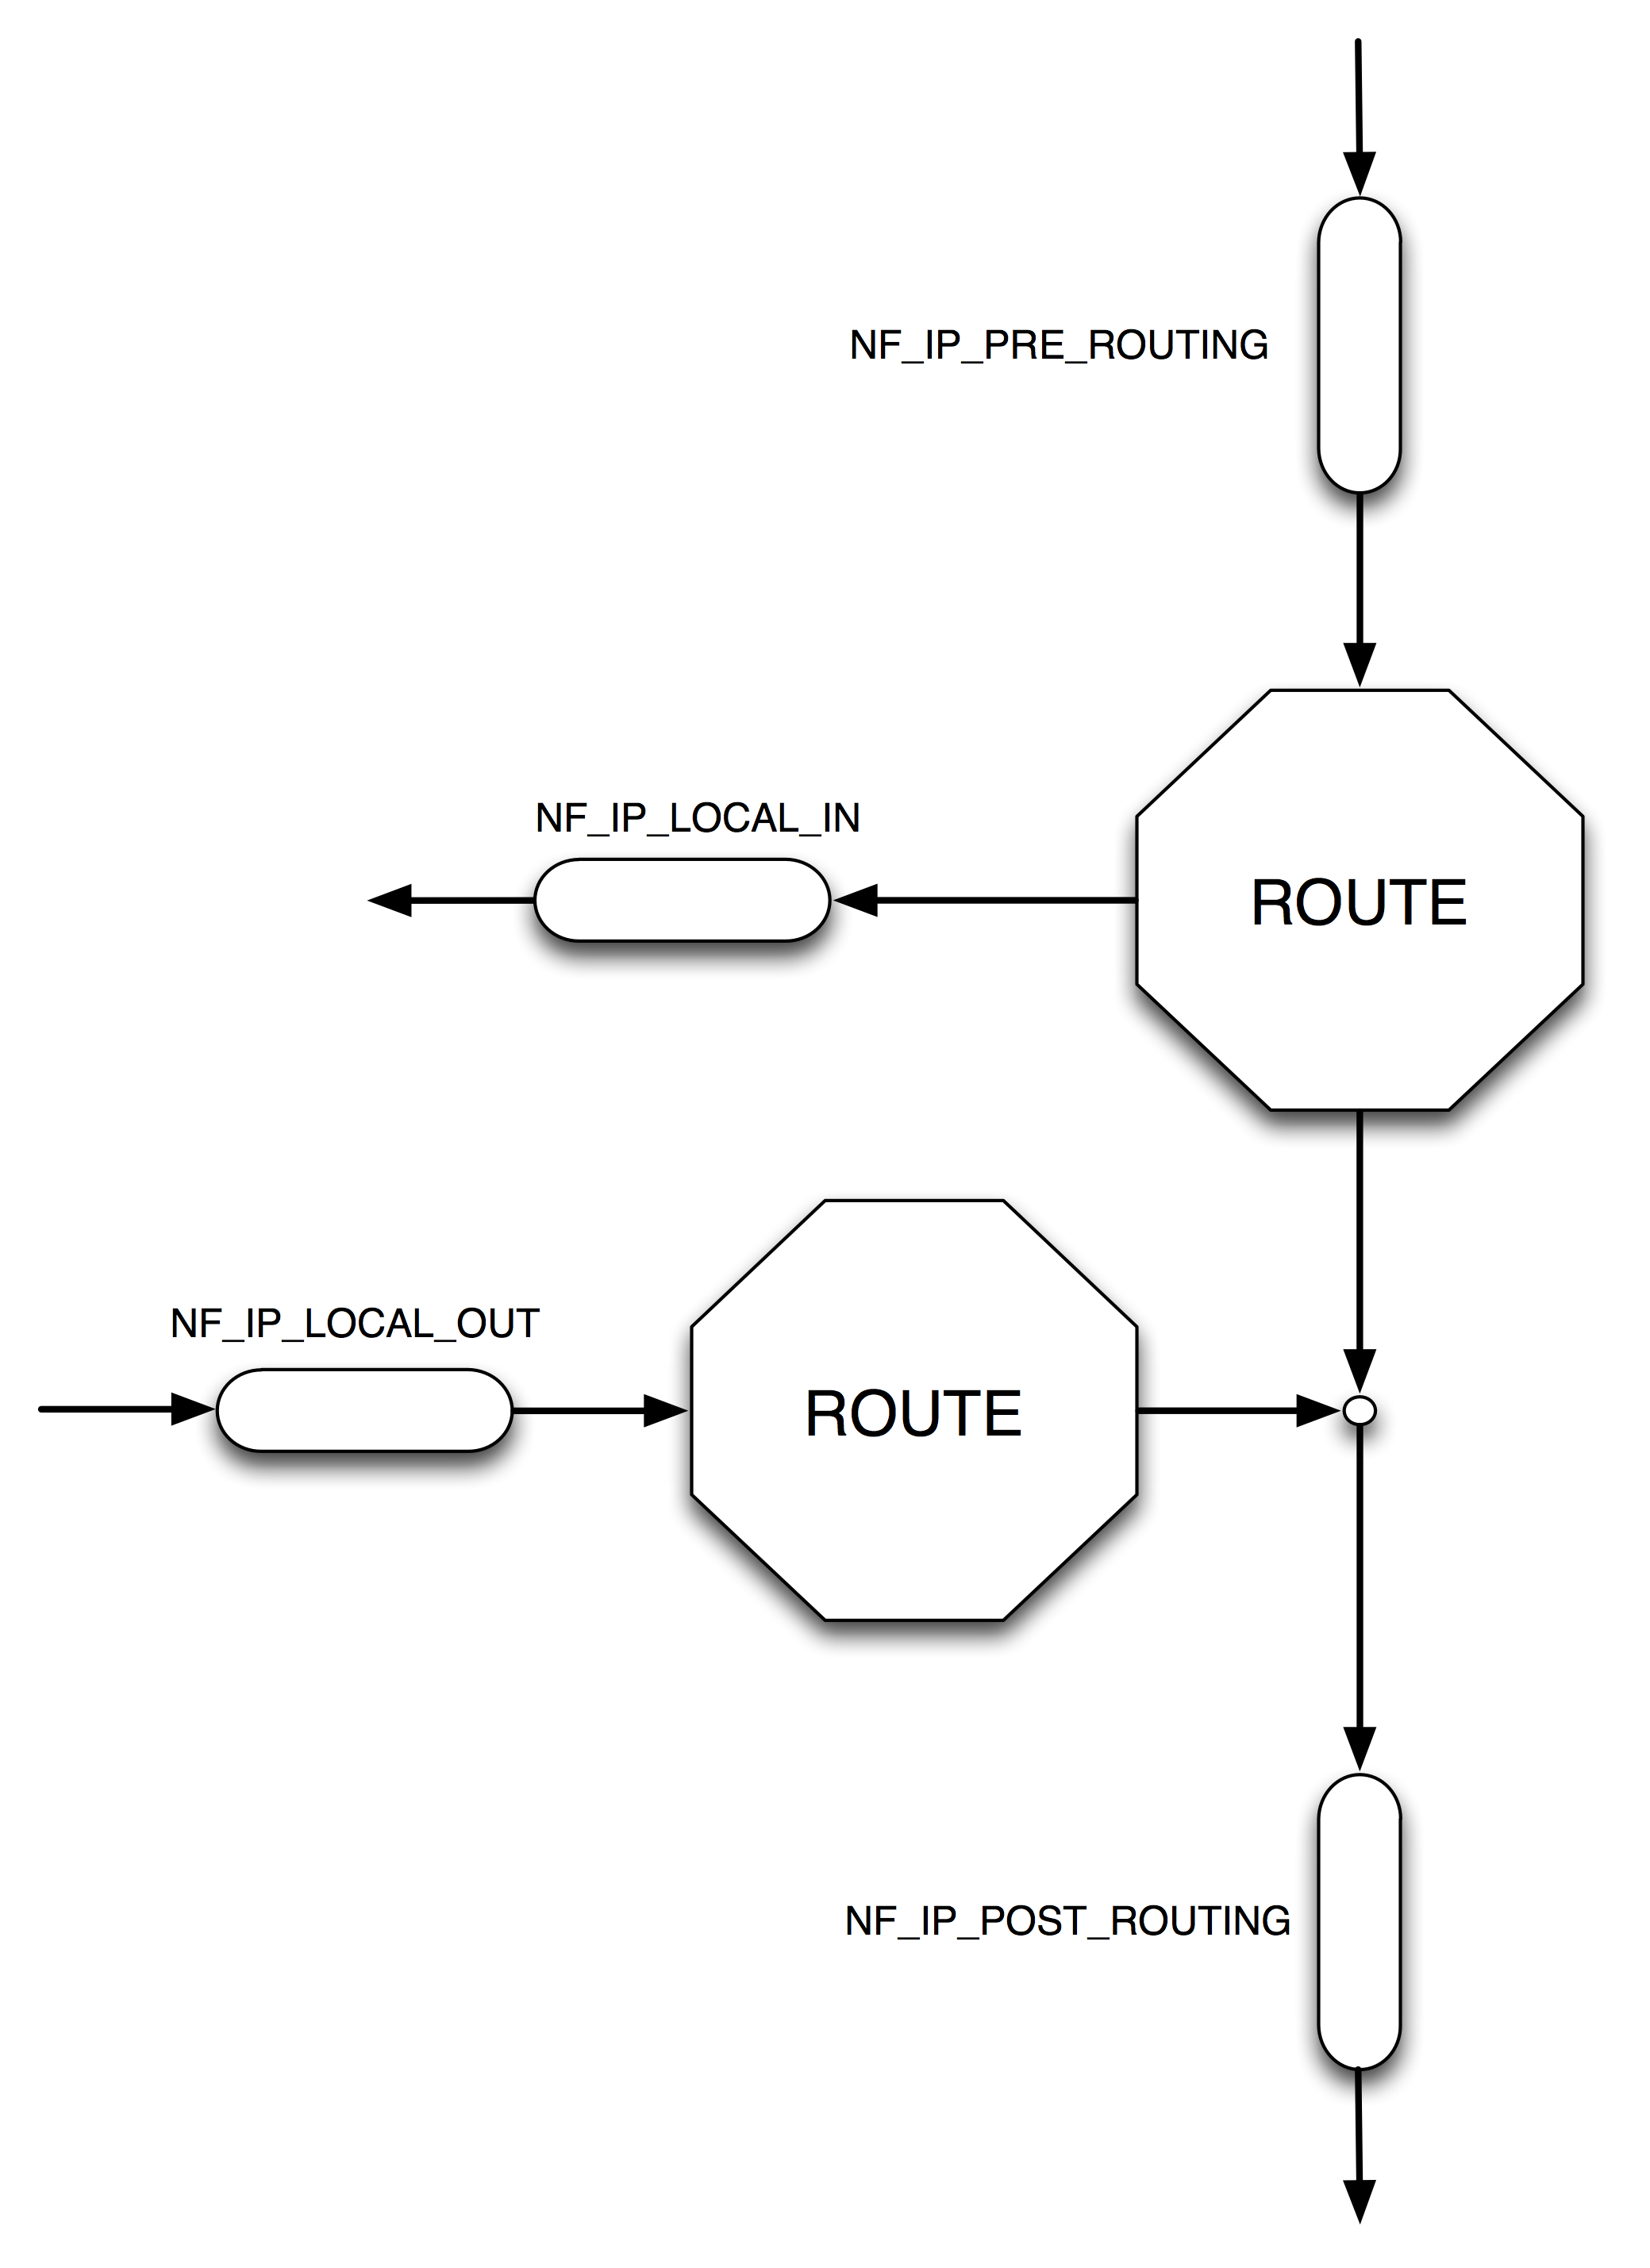
\includegraphics[totalheight=0.40\textheight]{images/hooks.png}
\caption{The packet is passed into \code{iptables}' hooks at certain points
  before and after routing.}\label{fig:hooks}
\end{figure}

The hook list object is a standard double linked list object used throughout the kernel. It's definition \verb|list_head| and utility functions are defined in \verb|include/linux/list.h| and allows for standard linked list functionality. A linked list is a perfect data structure in this case since there is no specific element indexing, but rather traversing through the list and calling all the available hooks. There are 6 hooks lists \figref{fig:hooks}. One for each of \verb|NF_INET_PRE_ROUTING| , \verb|NF_INET_LOCAL_IN|, \verb|NF_INET_FORWARD|, \verb|NF_INET_LOCAL_OUT|, \verb|NF_INET_POST_ROUTING|. By breaking the lists into one for each hook spot, on every spot where the hooks need to be called only the hooks responsible for that spot are iterated.

\begin{lstlisting}
extern struct list_head nf_hooks[NFPROTO_NUMPROTO][NF_MAX_HOOKS];
\end{lstlisting}

\subsection{Hook Adding}\label{hook_add}
The kernel attempts to add the hook object passed, by first creating a \verb|nf_hook_mutex| object, locking it until it has finnished the hook adding process. It then adds the given hook object by using the \verb|struct list_head list| as the reference pointer inside of the linked list but before adding it, loops through the list so that the list remains sorted by priority. That way when the hooks are called there is no need for sorting and the hooks with higher priority are called first. It unlocks the mutex and finally it adds the \verb|nf_register_hook| function to the modules API. This allows the function to be used from loaded modules. 

\begin{lstlisting}
int nf_register_hook(struct nf_hook_ops *reg)
{
	struct nf_hook_ops *elem;
	int err;

	err = mutex_lock_interruptible(&nf_hook_mutex);
	if (err < 0)
		return err;
	list_for_each_entry(elem, &nf_hooks[reg->pf][reg->hooknum], list) {
		if (reg->priority < elem->priority)
			break;
	}
	list_add_rcu(&reg->list, elem->list.prev);
	mutex_unlock(&nf_hook_mutex);
	return 0;
}
EXPORT_SYMBOL(nf_register_hook);
\end{lstlisting}

\subsection{Hook List Adding}\label{hook_list_adding}
The functionality to add several hooks at once also is available by letting the user provide an array of \verb|nf_hook_ops| and loop-add them to the linked list.

\begin{lstlisting}
int nf_register_hooks(struct nf_hook_ops *reg, unsigned int n)
{
	unsigned int i;
	int err = 0;

	for (i = 0; i < n; i++) {
		err = nf_register_hook(&reg[i]);
		if (err)
			goto err;
	}
	return err;

err:
	if (i > 0)
		nf_unregister_hooks(reg, i);
	return err;
}
\end{lstlisting}

\subsection{Hook And Hook-List Removing}\label{hook_removing}
The hooks can also be removed from the linked list in similar fashion to the way they are added.

\begin{lstlisting}
void nf_unregister_hook(struct nf_hook_ops *reg);
void nf_unregister_hooks(struct nf_hook_ops *reg);
\end{lstlisting}

\subsection{Hooks Processing}\label{hooks_processing}
Finally there exist facilities inside \verb|netfilter.h| that allow the kernel to process the hooks that are registered at the various steps. Many are in the form of macros that add certain small functionality before the function \verb|nf_hook_slow| is called. This function iterates through all the hooks registered for the current step, executes them and proceeds according to the result returned by the hook.

\begin{lstlisting}
int nf_hook_slow(u_int8_t pf, unsigned int hook, struct sk_buff *skb,
		 struct net_device *indev, struct net_device *outdev,
		 int (*okfn)(struct sk_buff *), int thresh);
\end{lstlisting}


